\documentclass{article}
\usepackage{graphicx}
\title{Wyznaczanie charakterystyki prądowo-napięciowej diody
rezonansowo-tunelowej (RTD) oraz zastosowanie przybliżenia
adiabatycznego do wyznaczenia zjawiska kwantyzacji konduktancji
w kwantowym kontakcie punktowym (QPC).}
\author{Marta Wleklińska}
\input{setup}
\usepackage[margin=2cm]{geometry}
\usepackage{polski}
\date{\today}

\begin{document}

\maketitle

%%%%%%%%%%%%%%%%%%%%%%%%%%%%%%%%%%%%%%%%%%%%%%%%%%%%%%%%%%%%%
\section{Cel ćwiczenia}
Ćwiczenie polega na zbadaniu transportu elektronowego w diodzie rezonansowo--tunelowej oraz w kwantowym kontakcie punktowym w nanodrucie 2D.
%%%%%%%%%%%%%%%%%%%%%%%%%%%%%%%%%%%%%%%%%%%%%%%%%%%%%%%%%%%%%
\section{Wstęp}
%%%%%%%%%%%%%%%%%%%%%%%%%%%%%%%%%%%%%%%%%%%%%%%%%%%%%%%%%%%%%
Jedną z metod obliczeniowych używanych w celu opisania układu w strukturach o zmiennym potencjale jest metoda macierzy transferu. 
Polega ona na podziale obszaru o zmiennym potencjale na $N$ cienkich warstw, w których potencjał jest aproksymowany jako stały.
Dla każdej z tych warstw rozwiązywane jest niezależne od czasu równanie Schr{\"o}dingera
\begin{equation}
    -\frac{\hbar^2}{2m^*_n}\dv[2]{z}\psi_n(z)
 + U_n \psi_n(z) = E\psi_n(z),
 \end{equation}
 którego rozwiązaniem jest kombinacja liniowa fal płaskich: fal padających i odbitych. 
 Należy jednak zaznaczyć, że funkcja falowa oraz jej pochodna (ważona odwrotnością masy efektywnej) muszą być ciągłe na granicy każdej warstwy, co prowadzi do warunku ciągłości:
 \begin{equation}
     \psi_n(z_n) = \psi_{n+1}(z_n), \quad
     \frac{1}{m_n^*}\dv{z}\psi_n(z_n) = \frac{1}{m^*_{n+1}}\dv{z}\psi_{n+1}(z_n),
 \end{equation}
 gdzie uwzględniamy również możliwość zmiennej masy efektywnej $m^*_n$ w kolejnych warstwach.
Warunki te można zapisać w postaci równania macierzowego z użyciem tzw. macierzy monodromii. 
Pozwala ona na powiązanie współczynników amplitudy fal w pierwszym i ostatnim obszarze. 
Na jej podstawie można obliczyć współczynniki transmisji i odbicia:
\begin{align}
     T = \frac{k_N m_1}{k_1 m_N}\frac{1}{|M_{1\rightarrow N, 11}|^2},\label{eq:trans}\\
     R = \frac{|M_{1\rightarrow N, 21}|^2}{|M_{1\rightarrow N, 11}|^2}, \label{eq:refl}
 \end{align}
gdzie $M_{1\rightarrow N}$ to całkowita macierz transferu opisująca cały układ od pierwszej do ostatniej warstwy.


%%%%%%%%%%%%%%%%%%%%%%%%%%%%%%%%%%%%%%%%%%%%%%%%%%%%%%%%%%%%%
\section{Wyniki}
%%%%%%%%%%%%%%%%%%%%%%%%%%%%%%%%%%%%%%%%%%%%%%%%%%%%%%%%%%%%%
\subsection{Dioda rezonansowo--tunelowa}
%%%%%%%%%%%%%%%%%%%%%%%%%%%%%%%%%%%%%%%%%%%%%%%%%%%%%%%%%%%%%
\subsubsection{Pojedyncza bariera}
%%%%%%%%%%%%%%%%%%%%%%%%%%%%%%%%%%%%%%%%%%%%%%%%%%%%%%%%%%%%%
Pierwszym krokiem była symulacja transportu elektronowego przez pojedynczą barierę potencjału, w celu przetestowania poprawności implementacji metody macierzy transferu.
Bariera była utożsamiana z cienką warstwą materiału o innej strukturze – przykładowo GaAs domieszkowanego Al, czyli Al$_{x}$Ga$_{1-x}$As. Dla rozpatrywanego przypadku $x = 0{,}3$, masa efektywna wynosiła:
\[
m^*_{\text{Al}_{0.3}\text{Ga}_{0.7}\text{As}} = 0.063 + 0.083 \cdot 0.3,
\quad
m^*_{\text{GaAs}} = 0.063.
\]
Na rysunku~\ref{fig:ex1 trans refl} przedstawiono zależności transmitancji i reflektancji obliczonych z równań~\eqref{eq:trans},~\eqref{eq:refl}. 
Na rysunku~\ref{fig:ex1 const mass} przyjęto stałą masę równą masie efektywnej GaAs, natomiast na rysunku~\ref{fig:ex1 non const mass} użyto różnej masy efektywnej w obszarze bariery.\\
% Pierwsza część ćwiczenia polegała na symulacji transportu elektronowego w diodzie rezonansowo--tunelowej.
% Najpierw jednak mogliśmy przetesować poprawność działania macierzy transferu dla prostrzego układu z pojedynczą barierą potencjału.
% Bariera była utożsamiana z inną warstwą materiału, czyli np. GaAs domieszkowanym Al.
% Dla każdego rozpatrywanego przedziału występowałą zatem inna masa efektywna $m^*_{\text{AlGaAs}} = (0.063 + 0.083 \cdot 0.3)$ oraz $m^*_{\text{GaAs}} = 0.063$.
% Na rysunku~\ref{fig:ex1 trans refl} ukazane zostały zależności transmitacji oraz reflektancji danymi wzorami~\eqref{eq:trans},~\eqref{eq:refl}.
% Na rysunku~\ref{fig:ex1 const mass} przyjęliśmy masę materiału bariery równą GaAs, a na rysunku~\ref{fig:ex1 non const mass} - masę Al$_{0.3}$Ga$_{0.7}$As.\\
%%%%%%%%%%%%%%%%%%%%%%%%%%%%%%%%%%%%%%%%%%%%%%%%%%%%%%%%%%%%%
\begin{figure}[htp!]
    \centering
\begin{subfigure}{.495\textwidth}
    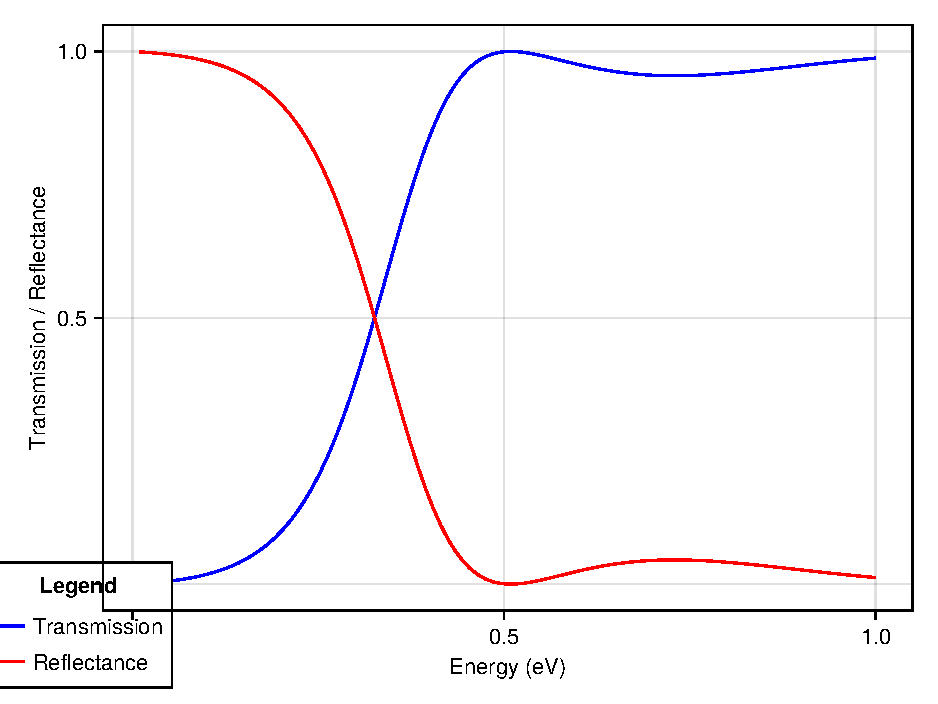
\includegraphics[width=1.0\linewidth]{ex1_trans_refl_const.pdf}
    \caption{}
    \label{fig:ex1 const mass}
\end{subfigure}
\begin{subfigure}{.495\textwidth}
    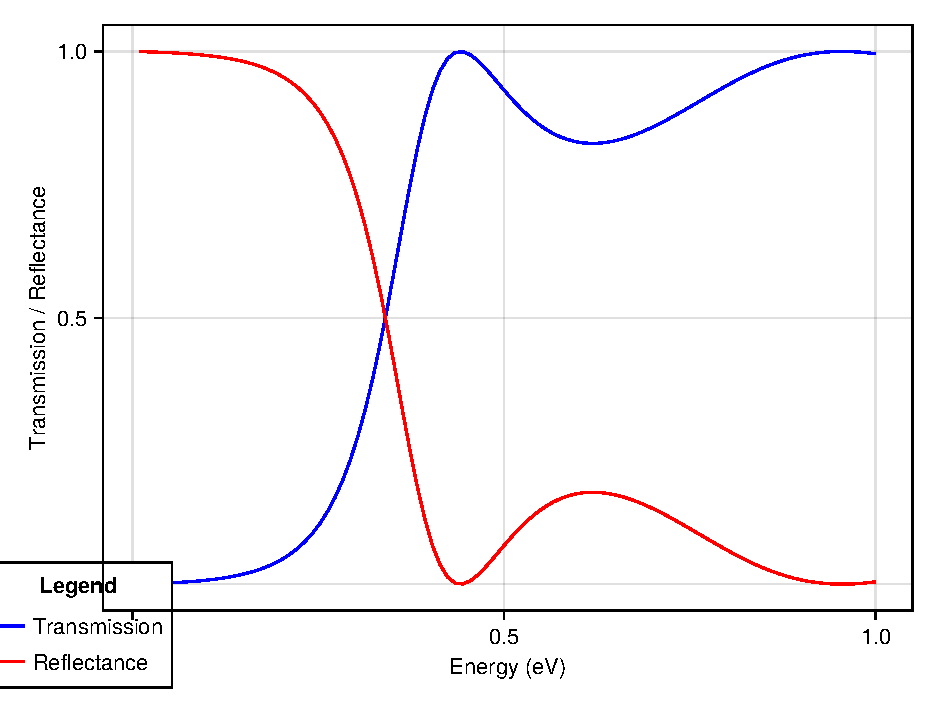
\includegraphics[width=1.0\linewidth]{ex1_trans_refl.pdf}
    \caption{}
    \label{fig:ex1 non const mass}
\end{subfigure}
\caption{Współczynnik transmisji i odbicia dla układu pojedynczej bariery przy~\textbf{(a)}~stałej masie w układzie, \textbf{(b)}~zmiennej masy w układzie}
\label{fig:ex1 trans refl}
\end{figure}
%%%%%%%%%%%%%%%%%%%%%%%%%%%%%%%%%%%%%%%%%%%%%%%%%%%%%%%%%%%%%
\\
Można zauważyć, że przy zmiennej masie bariera staje się bardziej zauważalna — po osiągnięciu maksimum transmitancji, dla wyższych energii współczynnik transmisji maleje szybciej niż w przypadku stałej masy.
%%%%%%%%%%%%%%%%%%%%%%%%%%%%%%%%%%%%%%%%%%%%%%%%%%%%%%%%%%%%%
\subsubsection{Podwójna bariera}
%%%%%%%%%%%%%%%%%%%%%%%%%%%%%%%%%%%%%%%%%%%%%%%%%%%%%%%%%%%%%
Dioda rezonansowo--tunelowa (RTD) to struktura składająca się z dwóch barier oddzielonych cienką warstwą materiału o niższym potencjale. 
W naszym przypadku były to dwie warstwy Al$_{0.3}$Ga$_{0.7}$As oraz studnia GaAs.\\
\\
Dla tej struktury również zastosowano metodę macierzy transferu, obliczając zależności współczynników transmisji i odbicia w funkcji energii — wyniki przedstawiono na rysunku~\ref{fig:ex2-trans-refl}.\\
%%%%%%%%%%%%%%%%%%%%%%%%%%%%%%%%%%%%%%%%%%%%%%%%%%%%%%%%%%%%%
\begin{figure}[htp!]
    \centering
    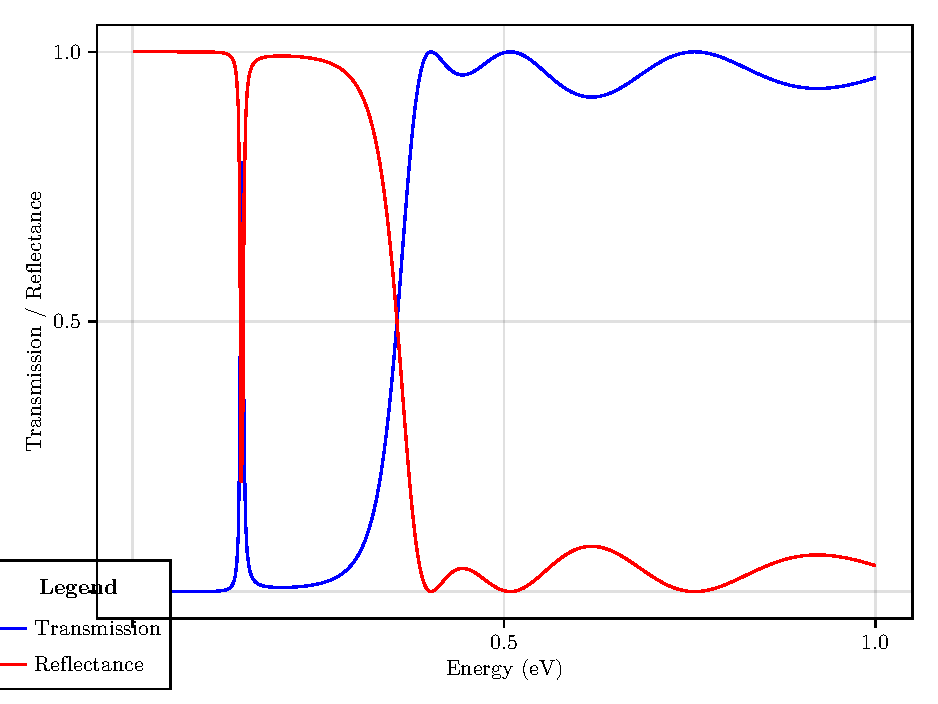
\includegraphics[width=0.7\linewidth]{ex2_trans_refl.pdf}
    \caption{Współczynnik transmisji i odbicia w funkcji energii przy założeniu zmiennej masy diody rezonansowo--tunelowej}
    \label{fig:ex2-trans-refl}
\end{figure}
%%%%%%%%%%%%%%%%%%%%%%%%%%%%%%%%%%%%%%%%%%%%%%%%%%%%%%%%%%%%%
\\
Charakterystyczną cechą jest występowanie ostrych maksimów transmitancji (rezonansów) dla energii mniejszych niż wysokość bariery.  
Dla wyższych energii obserwujemy oscylacje transmitancji i reflektancji, wynikające z interferencji fal odbitych i transmitowanych.
\subsubsection{Charakterystyka prądowo--napięciowa}
% Analiza diody rezonansowo--tunelowej również może obejmować charakterystykę prądowo napięciową.
% Do jej wyznaczenia, skorzystamy z formuły Tsu--Esakiego
% \begin{equation}
%     j = \frac{em^*k_{\text{B}}T}{3\pi^2\hbar^2}
%     \int_{0^{\infty}}\dd E_z \ \text{Trans}(E_z)\ln\left[\frac{1 + \exp\left(\frac{\mu_s - E_z}{k_{\text{B}}T} \right)}{1 + \exp\left(\frac{\mu_s - eV_{\text{bias}} - E_z}{k_{\text{B}}T}, \right)}\right]
% \end{equation}
% przy czym $\mu_s=0.087$~eV to potencjał chemiczny źródła, $V_{\text{bias}}$ to przyłożone napięcie, zaś $T=10$ to temperatura układu, a $\text{Trans}()$ to funkcja współczynnika transmisji w funkcji energii mogąca być wyznaczona metodą macierzy transferu.
% Należy zaznaczyć, że wprowadzając napięcie $V_{\text{bias}}$ profil energii potencjalnej się zmienia.
% Będzie on liniowo maleć aż w punkcie przyłożenie będzie mniejszy od wartości potencjału 
% Na rysunku~\ref{fig:ex2-current} uzyskana została charakterystyka prądowo--napięciowa diody korzystając  z powyższego wzoru.\\
Charakterystykę prądowo--napięciową diody RTD można obliczyć korzystając z formuły Tsu--Esakiego:
\begin{equation}
    j = \frac{em^*k_{\text{B}}T}{3\pi^2\hbar^2}
    \int_{0}^{\infty}\dd E_z \ \text{Trans}(E_z)\ln\left[\frac{1 + \exp\left(\frac{\mu_s - E_z}{k_{\text{B}}T} \right)}{1 + \exp\left(\frac{\mu_s - eV_{\text{bias}} - E_z}{k_{\text{B}}T} \right)}\right],
\end{equation}
gdzie $\mu_s = 0.087$~eV to potencjał chemiczny źródła, $V_{\text{bias}}$ to przyłożone napięcie, $T = 10$~K to temperatura układu, a~$\text{Trans}(E_z)$ to funkcja transmitancji wyznaczona wcześniej metodą macierzy transferu.\\
\\
Wprowadzenie napięcia $V_{\text{bias}}$ powoduje zmianę profilu potencjału — przyjmuje się, że spada on liniowo w obszarze struktury (przybliżenie rampy potencjału).
Na rysunku~\ref{fig:ex2-current} przedstawiono uzyskaną charakterystykę prądowo--napięciową.\\
%%%%%%%%%%%%%%%%%%%%%%%%%%%%%%%%%%%%%%%%%%%%%%%%%%%%%%%%%%%%%
\begin{figure}[htp!]
    \centering
    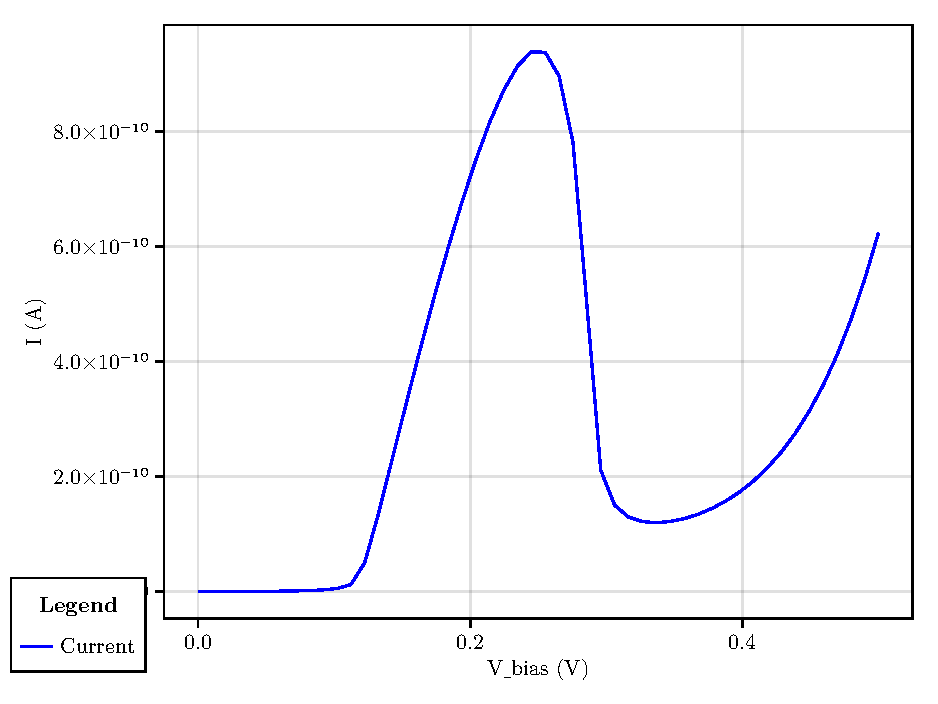
\includegraphics[width=0.7\linewidth]{ex2_current.pdf}
    \caption{Charakterystyka prądowo--napięciowa diody rezonansowo--tunelowej}
    \label{fig:ex2-current}
\end{figure}
%%%%%%%%%%%%%%%%%%%%%%%%%%%%%%%%%%%%%%%%%%%%%%%%%%%%%%%%%%%%%
\\
Krzywa posiada charakterystyczny kształt z obszarem ujemnego oporu różniczkowego. 
% Wynika on z faktu, że dla małych napięć energia rezonansu znajduje się w zakresie dostępnych stanów elektronowych w źródle i drenie, co umożliwia rezonansowe tunelowanie. 
Po przekroczeniu pewnego napięcia, rezonans wypada poza zakres stanów dostępnych w emiterze, co prowadzi do zmniejszenia prądu — pomimo wzrostu napięcia. 
%%%%%%%%%%%%%%%%%%%%%%%%%%%%%%%%%%%%%%%%%%%%%%%%%%%%%%%%%%%%%
\subsection{Transport w kwantowym kontakcie punktowym (QPC)} 
%%%%%%%%%%%%%%%%%%%%%%%%%%%%%%%%%%%%%%%%%%%%%%%%%%%%%%%%%%%%% 
W drugiej części ćwiczenia analizowany był transport elektronowy w kwantowym kontakcie punktowym (QPC), który modelowano jako przewężenie w dwuwymiarowym nanodrucie.\\
\\
Zadanie polegało na wyznaczeniu efektywnego potencjału $V_{\text{eff}}(x)$, z jakim oddziałuje elektron poruszający się w kierunku transportu ($x$), dla różnych stanów poprzecznych $n$. 
Potencjał generowany w układzie przy przyłożeniu napięcia~$V_g$ jest opisywany w postaci
\begin{equation}
    V(x, y) = f\left[x-l, y-b\right]
    +f\left[x-l, t-y\right]
    +f\left[r-x, y-b\right]
    +f\left[r-x, t-y\right],
\end{equation}
przy czym
\begin{equation}
    f(u,v) = \frac{eV_g}{2\pi \epsilon}\arctan \left(\frac{uv}{d\sqrt{d^2+u^2+v^2}}\right),
\end{equation}
gdzie $\epsilon$ to przenikalność elektryczna materiału, $l,r$ - położenia lewego i prawego brzegu bramki, a $t,b$ - położenia graniczne bramki w kierunku pionowym oraz $d$ to odległość pomiędzy bramkami a 2DEG.
Potencjał opisywany powyższą funkcją jest opisany w dwóch wymiarach, zatem skorzystaliśmy z przybliżenia adiabatycznego w obliczeniach.\\
\\
Na rysunku~\ref{fig:ex3-eff-pot} przedstawiono przykładowe profile efektywnego potencjału dla stanów $n=1$ do $n=5$.\\
%%%%%%%%%%%%%%%%%%%%%%%%%%%%%%%%%%%%%%%%%%%%%%%%%%%%%%%%%%%%% 
\begin{figure}[htp!]
    \centering
    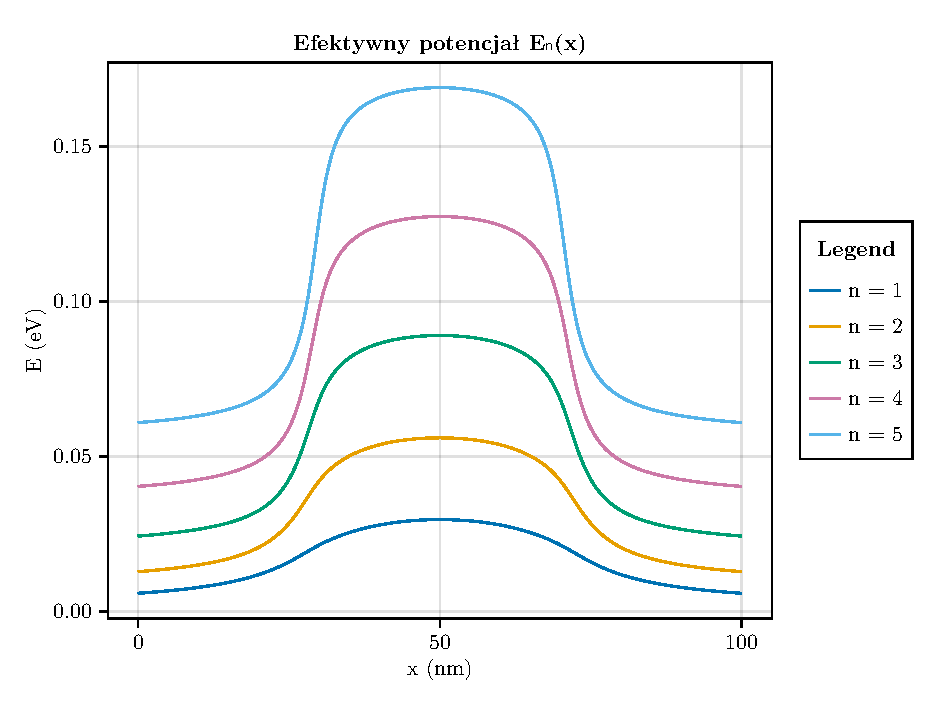
\includegraphics[width=0.7\linewidth]{ex3_potential.pdf}
    \caption{Profile kolejnych $n=5$ energii dla efektywnego potencjału }
    \label{fig:ex3-eff-pot}
\end{figure}
%%%%%%%%%%%%%%%%%%%%%%%%%%%%%%%%%%%%%%%%%%%%%%%%%%%%%%%%%%%%% 
\\
Na podstawie każdego z tych potencjałów można obliczyć współczynnik transmisji $T(E_n)$ metodą macierzy transferu.
Następnie mogliśmy wyznaczyć konduktancję całkowitą zgodnie z formułą Landauera: 
\begin{equation} 
G = \frac{2e^2}{h} \sum_n T_n(E).
\end{equation} 
Na rysunku~\ref{fig:ex3 conductance} pokazano otrzymane wartości konduktancji $G$ w funkcji energii padającego elektronu.\\
%%%%%%%%%%%%%%%%%%%%%%%%%%%%%%%%%%%%%%%%%%%%%%%%%%%%%%%%%%%%% 
\begin{figure}[htp!]
    \centering
    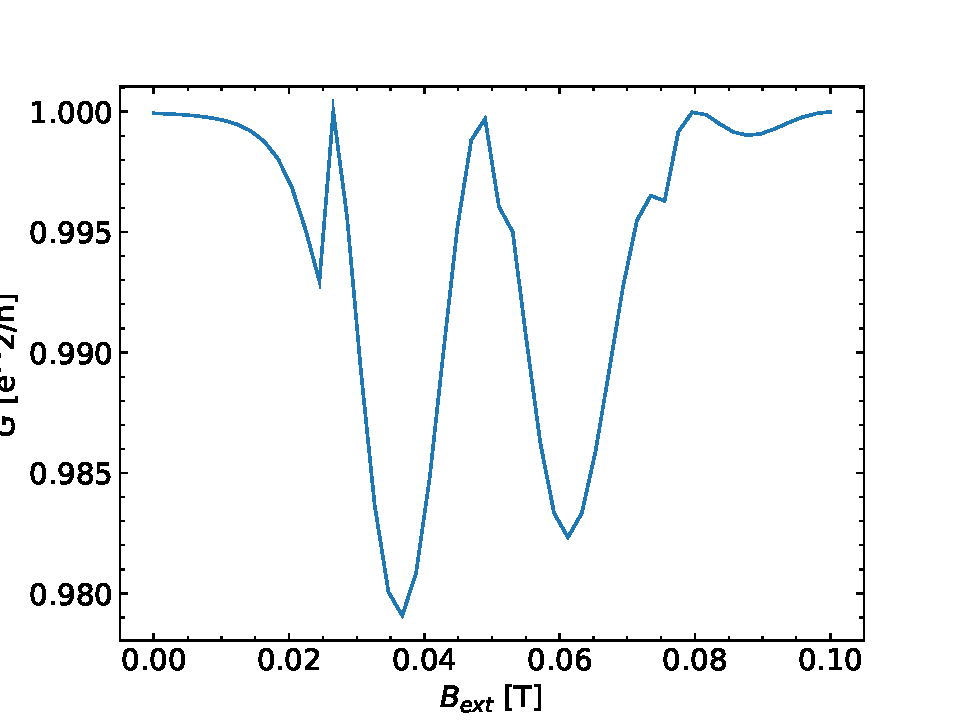
\includegraphics[width=0.6\linewidth]{ex3_conductance.pdf}
    \caption{Konduktancja w funkcji energii padającego elektronu wyznaczona dla QPC przy pomocy przybliżenia adiabatycznego}
    \label{fig:ex3 conductance}
\end{figure}
%%%%%%%%%%%%%%%%%%%%%%%%%%%%%%%%%%%%%%%%%%%%%%%%%%%%%%%%%%%%% 
\\
Zauważalne są charakterystyczne \textit{schodki}, czyli dyskretne wartości konduktancji w funkcji energii.
Zwiększając energię, dyskretne konduktancje są zwiększane.
Obserwowane zjawisko schodkowej konduktancji jest konsekwencją kwantowania liczby modów transmisyjnych – tylko skończona liczba stanów poprzecznych przyczynia się do przenoszenia ładunku, a każdy z nich wnosi dokładnie $\frac{2e^2}{h}$ do całkowitej konduktancji.
Przyjęto $n=5$ stanów w sumie.\\
\\
Dodatkowo zbadano zależność konduktancji od napięcia bramki $V_{\text{g}}$, dla danych energii Fermiego: $E=\{50, 100\}$~meV.
Na rysunku~\ref{fig:conductance vg} przedstawiono zależność konduktancji od $V_{\text{g}}$.
%%%%%%%%%%%%%%%%%%%%%%%%%%%%%%%%%%%%%%%%%%%%%%%%%%%%%%%%%%%%% 
\begin{figure}[htp!]
    \centering
    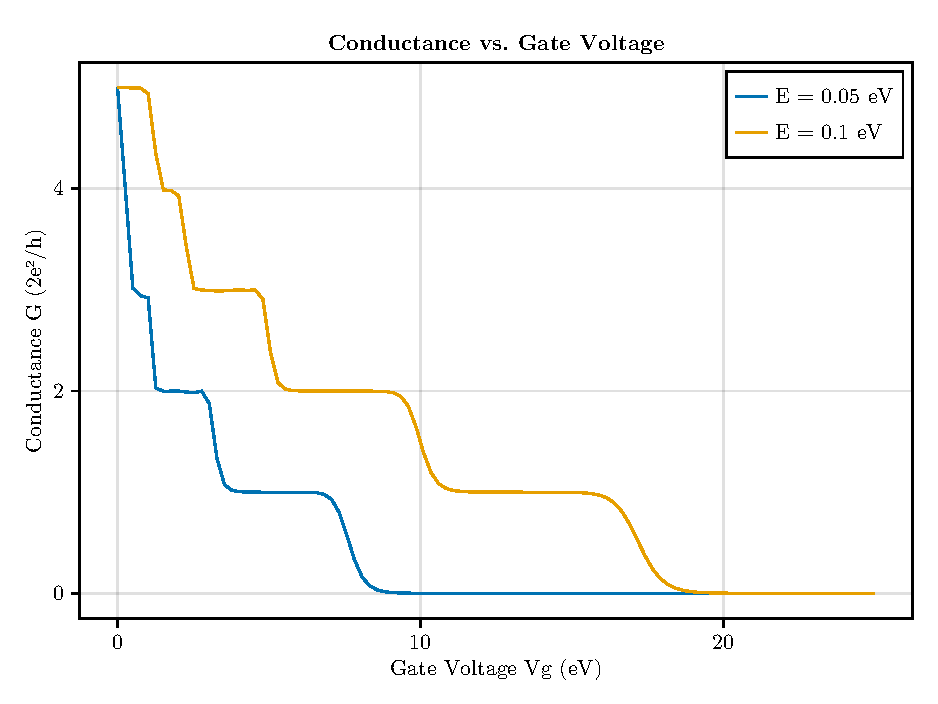
\includegraphics[width=0.6\linewidth]{ex3_conductance_vs_Vg.pdf}
    \caption{Konduktancja w funkcji napięcia $V_{\text{g}}$ na bramkach. 
    Wyniki dla $E = 50$~meV oraz $E = 100$~meV}
    \label{fig:conductance vg}
\end{figure}
%%%%%%%%%%%%%%%%%%%%%%%%%%%%%%%%%%%%%%%%%%%%%%%%%%%%%%%%%%%%% 
Zauważamy odwrotną zależność: im większe napięcie bramki~$V_{\text{g}}$, tym większy jest efektywny potencjał barierowy, co skutkuje wygaszaniem transmisji przez poszczególne kanały. 
Dla niższej energii Fermiego zauważamy szybsze gaśnięcie konduktancji.
%%%%%%%%%%%%%%%%%%%%%%%%%%%%%%%%%%%%%%%%%%%%%%%%%%%%%%%%%%%%%
\section{Podsumowanie}
%%%%%%%%%%%%%%%%%%%%%%%%%%%%%%%%%%%%%%%%%%%%%%%%%%%%%%%%%%%%%
Ćwiczenie polegało na zbadaniu dwóch nanourządzeń: diody rezonansowo--tunelowej oraz kwantowego kontaktu punktowego.
Do każdego z nich użyto metody macierzy transferu w celu znalezienia współczynnika transmisji przez bariery potencjału.
W pierwszej części dodatkowo wyznaczono charakterystykę prądowo--napięciową używając formuły Tsu--Esakiego.
W drugiej części z kolei badano konduktancję i jej \textit{schodkową} zależność od energii oraz przyłożonego napięcia. 


\end{document}
